% This is "sig-alternate.tex" V1.3 OCTOBER 2002
% This file should be compiled with V1.6 of "sig-alternate.cls" OCTOBER 2002
%
% This example file demonstrates the use of the 'sig-alternate.cls'
% V1.6 LaTeX2e document class file. It is for those submitting
% articles to ACM Conference Proceedings WHO DO NOT WISH TO
% STRICTLY ADHERE TO THE SIGS (PUBS-BOARD-ENDORSED) STYLE.
% The 'sig-alternate.cls' file will produce a similar-looking,
% albeit, 'tighter' paper resulting in, invariably, fewer pages.
%
% ----------------------------------------------------------------------------------------------------------------
% This .tex file (and associated .cls V1.6) produces:
%       1) The Permission Statement
%       2) The Conference (location) Info information
%       3) The Copyright Line with ACM data
%       4) Page numbers
%
% as against the acm_proc_article-sp.cls file which
% DOES NOT produce 1) thru' 3) above.
%
% Using 'sig-alternate.cls' you have control, however, from within
% the source .tex file, over both the CopyrightYear
% (defaulted to 2002) and the ACM Copyright Data
% (defaulted to X-XXXXX-XX-X/XX/XX).
% e.g.
% \CopyrightYear{2003} will cause 2002 to appear in the copyright line.
% \crdata{0-12345-67-8/90/12} will cause 0-12345-67-8/90/12 to appear in the copyright line.
%
% ---------------------------------------------------------------------------------------------------------------
% This .tex source is an example which *does* use
% the .bib file (from which the .bbl file % is produced).
% REMEMBER HOWEVER: After having produced the .bbl file,
% and prior to final submission, you *NEED* to 'insert'
% your .bbl file into your source .tex file so as to provide
% ONE 'self-contained' source file.
%
% ================= IF YOU HAVE QUESTIONS =======================
% Questions regarding the SIGS styles, SIGS policies and
% procedures, Conferences etc. should be sent to
% Adrienne Griscti (griscti@acm.org)
%
% Technical questions _only_ to
% Gerald Murray (murray@acm.org)
% ===============================================================
%
% For tracking purposes - this is V1.3 - OCTOBER 2002

\documentclass{sig-alternate-sigmod07}

\usepackage{hyperref}
\usepackage{cleveref}

\begin{document}
%
% --- Author Metadata here ---
%\conferenceinfo{ACM SIGMOD}{'07 Beijing, China}
%\CopyrightYear{2014} % Allows default copyright year (2000) to be over-ridden - IF NEED BE.
%\crdata{0-12345-67-8/90/01}  % Allows default copyright data (0-89791-88-6/97/05) to be over-ridden - IF NEED BE.
% --- End of Author Metadata ---
\makeatletter
\def\@copyrightspace{\relax}
\makeatother
\title{Short-term gas outliers detection using a hybrid ARIMA and Artificial neural network model}
%
% You need the command \numberofauthors to handle the "boxing"
% and alignment of the authors under the title, and to add
% a section for authors number 4 through n.
%
\numberofauthors{2}
\author{
% You can go ahead and credit any number of authors here,
% e.g. one 'row of three' or two rows (consisting of one row of three
% and a second row of one, two or three).
%
% The command \alignauthor (no curly braces needed) should
% precede each author name, affiliation/snail-mail address and
% e-mail address. Additionally, tag each line of
% affiliation/address with \affaddr, and tag the
% e-mail address with \email.
%
% 1st. author
\alignauthor
Maarten van Someren\\ %\titlenote{Dr.~Trovato insisted his name be first.}
       \affaddr{Universiteit van Amsterdam}\\
       \affaddr{Science Park 107}\\
       \affaddr{Amsterdam, The Netherlands}\\
       \email{m.w.vanSomeren@uva.nl}
% 2nd. author
\alignauthor
Marco De Nadai\\
       \affaddr{Universita' degli studi di Trento}\\
      \affaddr{Master's student}\\
       \email{marco.denadai@studenti.unitn.it}
}
\maketitle
\begin{abstract}
%in the last row, present the error RMSE

The focus of this paper is on building a robust outlier detection and prediction system, which relies on a hybrid Artificial neural network (ANN) and ARIMA model. ARIMA is suitable for linear prediction and ANNs are suitable for non-linear prediction. It is proved that together they can model the complex non-linear relationship between weather forecast variables and the gas consumption. The system labels outliers, which can be reported to the building manager. He can further analyse and fix the HVAC system minimizing in this way the energy waste. 
The hybrid system was tested with different buildings, predicting the short-term (hourly) gas consumption with a RMSE of $7.995$ and detecting all the outliers without the necessity of possessing the previous examples of anomalies.

\end{abstract}

\keywords{Energy forecasting, Time series, Artificial neural networks, ARIMA models, outliers, outliers detection, gas consumption prediction, energy forecast}

\section{Introduction}

Energy consumption in buildings is one of the fastest growing sectors. It is measured that the amount of energy consumed in European buildings (households and services) is about $41\%$ of the total energy consumption \cite{Eurostat2013}. Studies and states' directives about minimizing energy consumption and using renewable energy increased steadily with the reduction of fossil fuels, the border frictions with eastern countries like Russia, and the increase of various environmental problems. With this in mind, the European union, with a recent directive \cite{Directive2009}, has the target to raise EU energy consumption produced from renewable resources to $20\%$, to reduce by $20\%$ the EU greenhouse gas emissions and to improve by $20\%$ the EU's energy efficiency. This means investments to re-qualify old buildings, new country laws, energy diagnosis, but also new efficiency systems from the used appliances.

Forecasting energy demands has become one of the major research field in the energy departments because it can help gas utilities but also companies and families. Gas utilities buy gas from pipeline companies on a daily bases, so they need to know the needs in advance to be competitive.  Companies and families have the aim of reducing the energy consumption and increase efficiency. \\
Lately, big companies like Google also have shown their interest in this new market, developing thermostats which automatically control the house climate basing the decisions on the schedule of the users. Nest, a company acquired by Google, declared that customers saved the 11.3\% of AC-related energy usage without compromising comfort \cite{GoogleNest2}, thanks to the automatic learning implemented in their thermostats. If on one hand the automatic thermostat program setting based on the people behaviour, can help them to save money, anomaly detection can decrease even more the energy consumption. These anomalies usually have a large impact on the final consumption and if caused by deficiency, they represents a huge and easy fixable problem. 

In this paper an automatic outlier detection system is proposed, where days/hours with abnormally high and low energy consumption are labelled and reported to the building manager. He can further analyse and fix the HVAC system minimizing the energy waste caused by the outliers. The outlier detection system presented is based on predictions made by a hybrid ARIMA-ANN, which can model linear and non-linear behaviour of the data with very reliable results, and a comparison between the predicted value/trend and the actual one to find outliers. 

\subsection{What is an outlier}
An outlier, by definition \cite{hawkins1980identification}, is an observation which deviates significantly from other observations so that it creates suspicion that it was created by different dynamics. Outliers can have distinct main reasons: 
\begin{enumerate}
  \item Defective system (e.g. a defective heater in a room).
  \item Bad human behaviour (e.g. people who leave open the window in a room while the system is trying to heat it).
  \item Defective monitoring system, where the system monitors different values from the real one, due to a malfunction, computing process errors or a recording negligence. 
\end{enumerate}

Outliers are also referred to as abnormalities, deviants, novelties or anomalies in the data mining and statistics literature.

As can be seen in \cref{fig:outlierTypes} there are two main types of outliers unusual data point (e.g. a sudden jump of the energy consumption), or an unusual pattern of changes (e.g. a defective heater that lasts for days). The latter scenario is very challenging and not easily detectable.

\begin{figure}[h!]
\centering
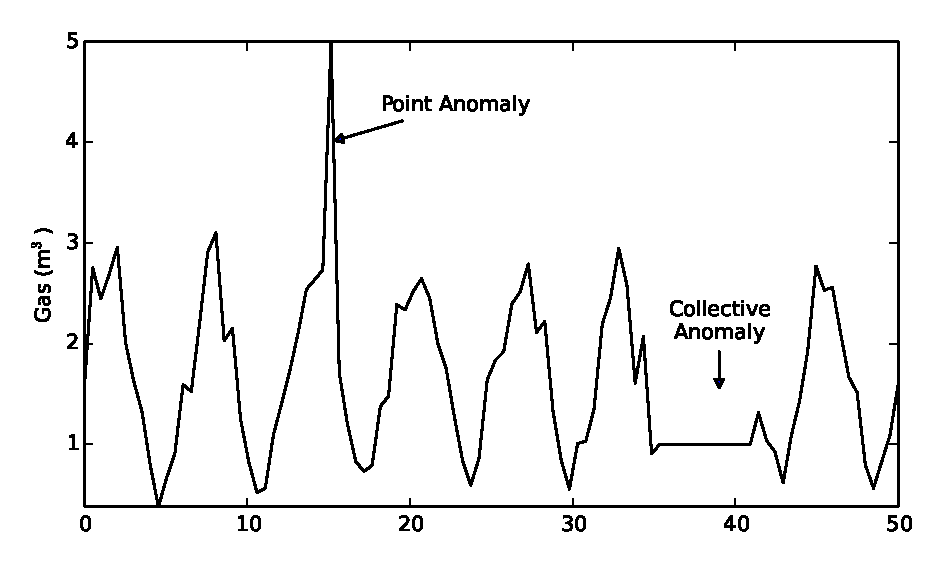
\epsfig{file=images/outlierTypes.eps, width=\columnwidth}
\caption{Different types of outliers. On the left an unusual data point is presented, on the right an unusual pattern of changes can be recognized if compared to the other days shape.}
\label{fig:outlierTypes}
\end{figure}

\section{Related work}
In order to have an excellent anomaly detection, a very accurate prediction model is necessary. This section will review some prediction methods as well as some outlier detection algorithms.

Traditionally, several techniques have been used for energy use forecasting, but it is needed to differentiate between short-term, medium-term and long-term energy forecasting. The former usually refers to prediction with a horizon of hours or days, the second refers to weeks, the latter refers to monthly or annual horizon. Long-term forecasting usually deals with data that rarely presents significant distortions and irregularities, so they have a small effect on the overall value. On the contrary, short-term forecasting has to deal with irregularities and sudden changes of the values (due to weather changes, human behaviour, etc.). 

There are essentially five types of prediction models \cite{zhao2012review}: Engineering methods, Statistical methods, Artificial Neural networks, Support Vector Machines and Grey models. Engineering methods use physical principles to calculate thermal dynamics and energy behaviour of the building, Statistical methods build empirical models to apply a regression to time series of values, Neural networks try to predict energy using an artificial intelligence network of interconnected neurons, Support vector machines are based in a machine learning algorithm and Grey models apply a mixture of the models. All the principal methods are extensively reviewed in \cite{zhao2012review} and \cite{hippert2001neural}. 

Several techniques have been traditionally applied for energy use forecasting, and among the statistical methods Kalman filtering and ARIMA/ARMAX time-series techniques are the most famous. 

The first reports about applications of Artificial Neural Networks (ANNs) were published in the early 1990's \cite{czernichow1996short}. Since then the number of publications increased steadily. Kalogirou et la. \cite{kalogirou2006artificial} used back propagation neural networks to predict the required heating load of 225 buildings, Ekici and Aksoy used the same model t predict building heating loads in three-buildings. Nizami and Al-Garni \cite{JaveedNizami19951097} tried a simple feed-foward NN and related the electric energy consumption to weather data and population, Taylor and Buizza \cite{taylor2002neural} used an ANN with weather data (51 variables) to predict load of 10 days ahead. Gonzales \cite{gonzalez2005prediction} built an ANN to predict hourly energy consumption.
Some researchers tried to specialize the ANNs: Neto and Fiorelli \cite{neto2008comparison} compared generic ANNs with working days ANNs and week-end ANNs, Lazzerini and Rosario \cite{d2012neural} specialized them to predict electric lighting with weather data. 

Some researchers tried also to apply a hybrid model to increase the performance of the ANN. One example above all is \cite{zhang2003time} which applied a hybrid ARIMA and neural network model to forecast electricity use, another one is \cite{khashei2010artificial} who improved the previous one. This paper is based also on his work.

Until now only electric forecasting was presented, because the majority of the existing forecasters are related to electric forecasting. There are only few of them are about natural gas forecasting: Brown et al.\cite{brown1995development} built one of the first predictor for natural gas consumption and Khotanzad et al \cite{khotanzad2000combination} developed a two stage system ANN with very good results.

Even if ANNs might outperform traditional methods, the researchers are not still convinced about the results of the ANNs in this field. Nevertheless it is also stated that ``a significant portion of the NN research in forecasting and prediction, lacks validity" \cite{adya1998ective} and that most of the papers seems misspecified models that had been incompletely tested (no standard benchmarks, no synthetic data, etc.) \cite{hippert2001neural}. This paper will try to avoid these mistakes.

Outlier detection system is a wide area from introduction detection systems to fraud detection systems, from law enforcement systems to earth science anomaly detection systems. Talking about energy consumption outlier detections, usually literature is based on the Gaussian error theory, stating that when the measurement accord with normal distribution, the probability that the residual falls in three times the variance is more than $99.7\%$. Therefore the residuals falling outside it, can be considered outliers. In \cite{ferdowsi2013neural} the author further improved this system considering a rolling moving window median which seems to improve the results when the distribution is not fixed. Other outlier detection mechanisms are based on supervised classifications using trees, ANNs and other different algorithms, thanks to the possession of previous examples of anomalies.
The last category of outliers detection system is represented by unsupervised methods like clustering, where an algorithm tries to find similarities between points/trends and cluster them into groups, calculating the distance between them. A cluster is good when the intra-cluster distance is minimized and the intra-cluster distance is maximized. Popular methods in this group are $k$-means, one-class SVM and self-organizing maps. They are very difficult to apply in time-series and the results are not usually excellent after it. For this reason they not considered in this paper.


\section{Proposed solution}

It can be seen that in academic and industry research, linear regression-based systems are the standard ``de facto" of energy forecasting and in recent works this problem is treated by combining weather forecast data. However, this relationship is clearly non-linear \cite{hippert2001neural}. Consequently, even if some papers have good results with measured datasets, these systems cannot adequately capture the relationship in all the situations and data. Since ANNs are the state of the art technique of many machine learning problems where there are complex non-linear hypothesis, the proposed solution is composed by a \textit{multilayer feed-foward} neural network with \textit{backpropagation}. This model is applied to the dataset and the outlier detection will be built on top of it. All the points far from the predicted value of the ANN, will be considered outliers.

\subsection{Experimental data}
The energy consumption datasets used are collected by Ebatech\footnote{http://www.ebatech.nl} in different buildings of the Hogeschool van Amsterdam\footnote{http://www.hva.nl/}. These buildings are located in Amsterdam, the capital city of The Netherlands. This city has an oceanic climate, strongly influenced by the North Sea. Winters are cold and summers are rarely hot. It is characterized by the common presence of rain and wind.\\
Ebatech collected different types of features in each buildings, with different granularity. For this project three buildings are used: \textit{HvA 740 - NTH}, \textit{Hva 882 - WBW} and \textit{Hva 761 - KMH}. In these buildings the company collected the energy consumptions, the gas consumptions as other variables.

\begin{table}
\centering
\caption{Buildings used}
\label{tab:dataset}
\begin{tabular}{|c|c|l|} \hline
Building name&Date interval&Number of rows\\ \hline\hline
HvA 740 - NTH & 01/2008 - 03/2014 & $54.725$\\ \hline
Hva 761 - KMH & 01/2008 - 03/2014 & $54.744$\\ \hline
Hva 882 - WBW& 01/2008 - 03/2014 & $54.647$\\ \hline
\end{tabular}
\end{table}

The weather data was collected by KNMI\footnote{Koninklijk Nederlands Meteorologisch Instituut http://www.knmi.nl} in Schipol, a Dutch city around 16 km far from the tested buildings. The available data consists in over 21 variables hourly collected. The proposed solution only uses few of them, as explained in the \cref{sec:datapreprocessing}, and they are used as forecast values: the measured weather conditions are linked to the previous hour of energy consumptions. It is necessary to consider that there will be an error in the built model, since the weather data is collected in a different location from the buildings positions and in practice the error will be larger than those obtained in this simulation, due to the effect of the weather forecast uncertainty \cite{douglas1998impacts, ranaweera1996effect}. The advice is to keep it in mind before applying the methods contained in this paper with days forecasting.

\subsubsection{Data analysis}
\label{sec:dataAnalysis}

The available dataset is conform to the nine characteristics of a good dataset as outlined by to Few \cite{few2009now}:
\begin{description}
\itemsep0em
  \item[Volume] As demonstrated in \cref{tab:dataset}, the dataset seems adequately large to train an ANN and test the results.
  \item[Historical] The dataset covers a very large period ranging more than 5 years, allowing to see similar patterns even with different yearly/seasons behaviour (one year could be different from another one for external factors like weather or building use). 
  \item[Consistent] The dataset of the selected buildings and for the variables that will be used, is consistent.
  \item[Multivariate] The dataset is composed by more than 50 variables, measuring the different behaviours of the buildings and the weather.
\item[Clean-Atomic] The dataset, after a minimal preprocessing, is clean and atomic. Some errors (outliers) were present on the data, but they were selected and deleted before the use.
\item[Clear] The dataset of the selected buildings and for the variables that will be used, is clear. The only problems were found on the not used variables: although they could be very useful, it was not possible to contact the buildings energy managers in order to understand them, for this reason they were excluded.
\item[Richy Segmented] The dataset can be segmented in several meaningful segments like gas consumption, electric consumption, water consumption, number of people using the buildings, etc.
\end{description}

The gas consumption data is highly seasonal: daily and weekly cycles are quite perceptible, as it can be seen from \cref{fig:monthlyTGas} and \cref{fig:dailyBehaviour}. From the latter the weekly behaviour is clear: the last two days of the week (Saturday and Sunday) are completely different from the others and Monday seems a bit different from the rest of the days. Everyday, around 4:00-5:00 AM, the system seems to react turning on the heating system, where in the previous hours of the night it seems only keeping a minimum temperature. The system reveals us that after a couple of hours, it decreases the consumption again.
In \cref{fig:monthlyTGas} the Temperature has a clear daily/hourly relation with the gas consumption while in \cref{fig:monthlyGasElectr} the electric consumption is shown to be very smoothed and more regular than the gas one.


\begin{figure}[h!]
\centering
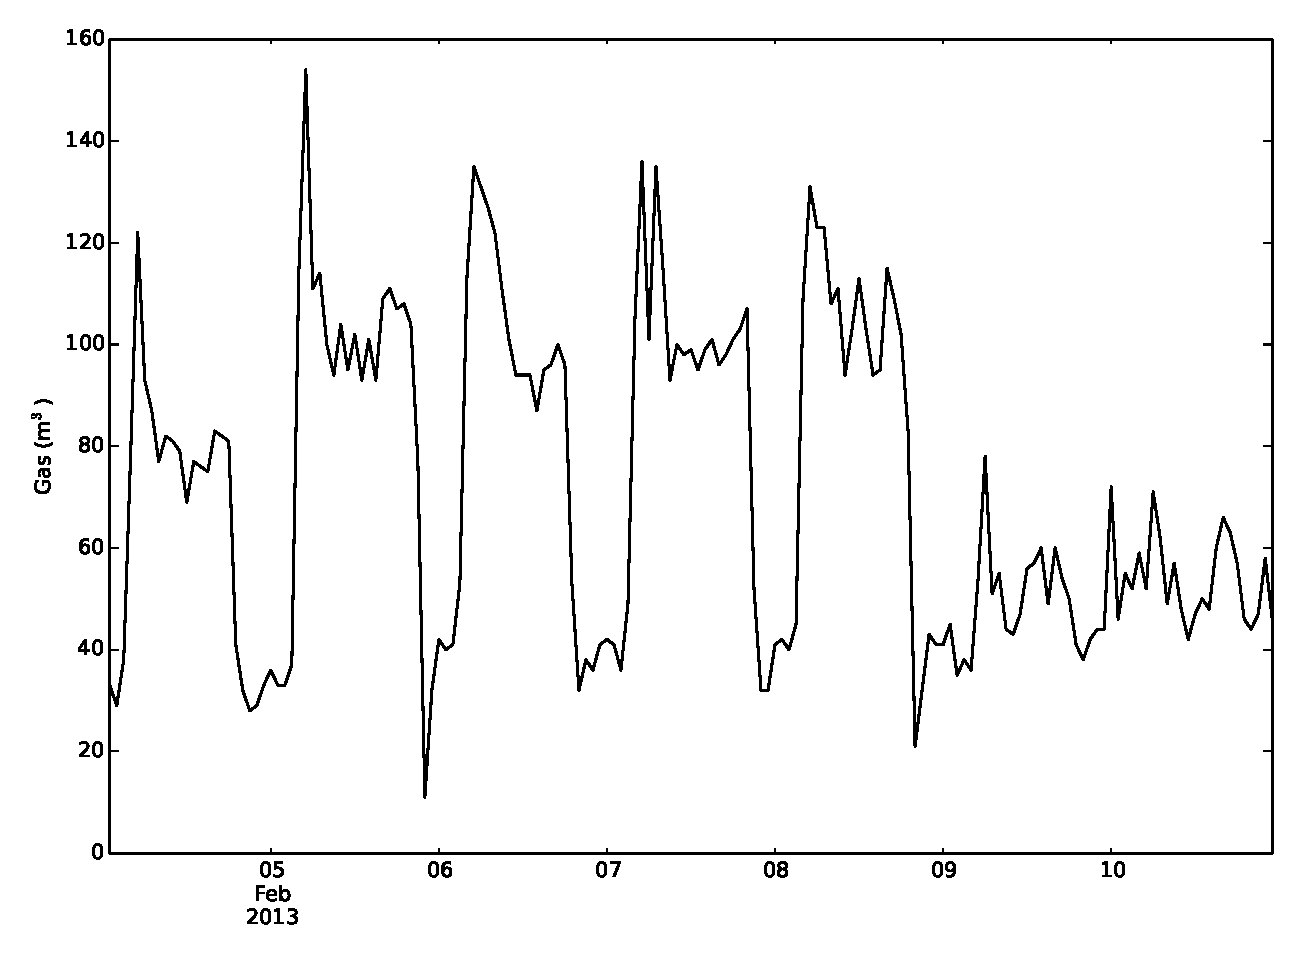
\epsfig{file=images/dailyBehaviour.eps, width=\columnwidth}
\caption{Typical weekly and daily gas consumption behaviour. The weekly pattern can be noticed by observing that the last two days of the week (Saturday and Sunday) have a completely different shape than the others. During the week, the daily behaviour is very similar, with one peak around 4:00-5:00 AM.}
\label{fig:dailyBehaviour}
\end{figure}

\begin{figure}[h!]
\centering
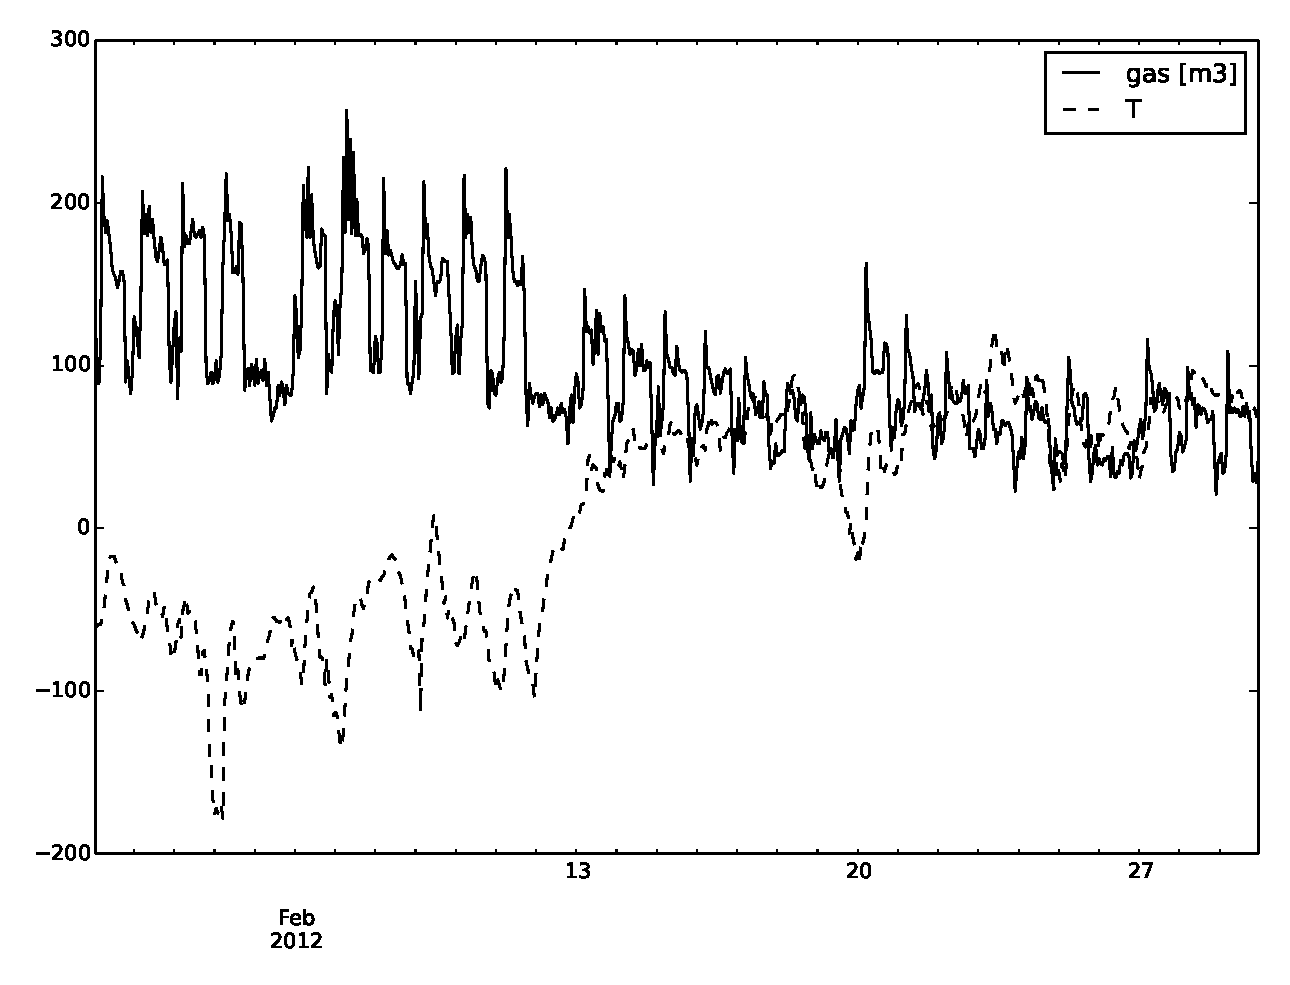
\epsfig{file=images/monthlyTGas.eps, width=\columnwidth}
\caption{Typical monthly gas consumption behaviour and its relation with the temperature}
\label{fig:monthlyTGas}
\end{figure}

\begin{figure}[h!]
\centering
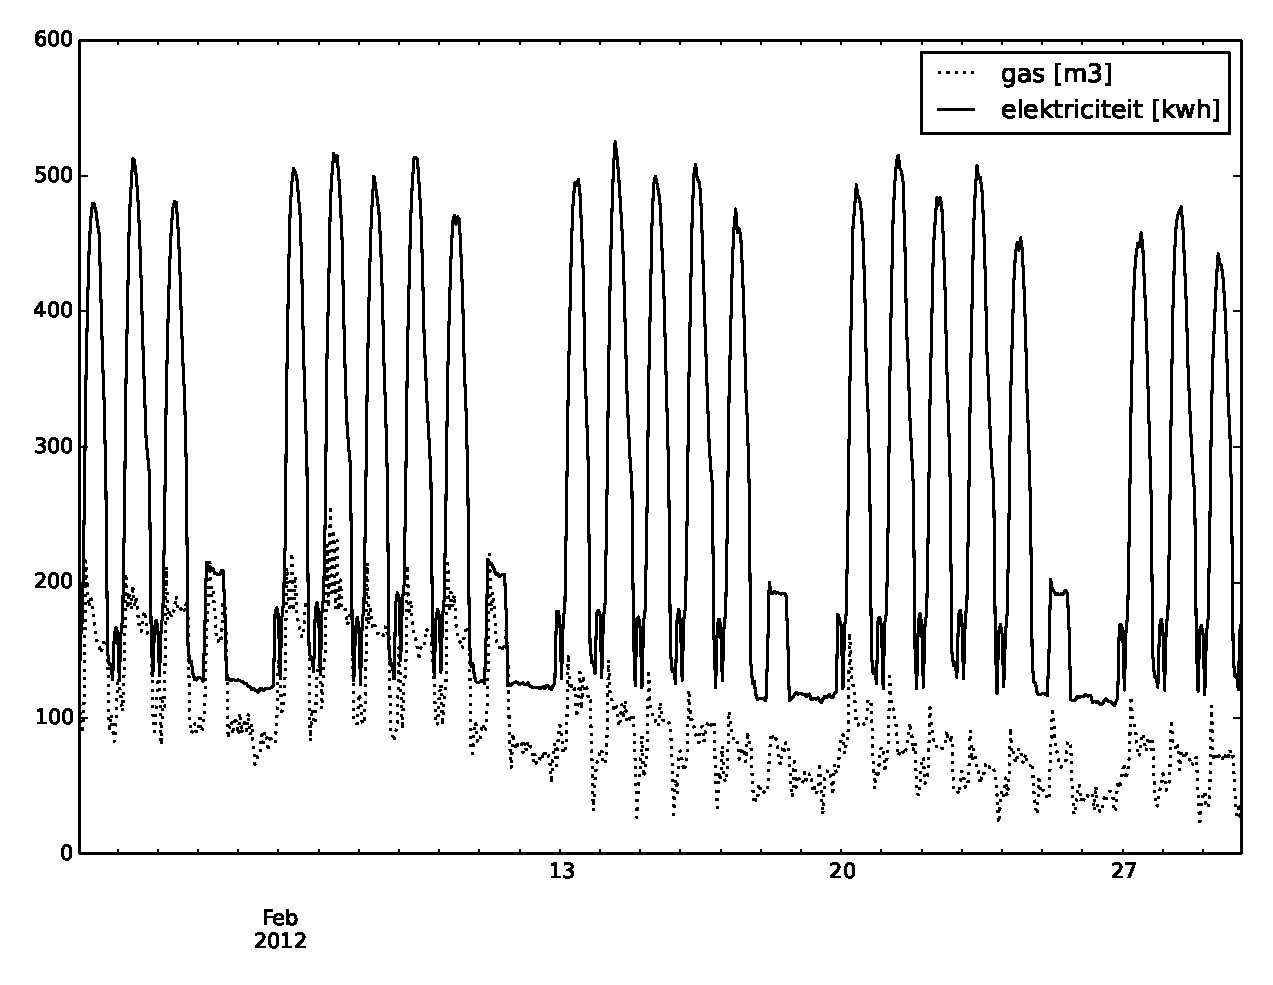
\epsfig{file=images/monthlyGasElectr.eps, width=\columnwidth}
\caption{Relation between electric and gas consumption}
\label{fig:monthlyGasElectr}
\end{figure}


\subsubsection{Data preprocessing}
\label{sec:datapreprocessing}

Since NNs are sensitive to missing values and irregularities, some data considered evident outliers will be removed, nevertheless it needs to be considered that since it was not possible to contact the buildings manager, it was not possible to remove other outliers. For this reason the ANN training was done with not entirely perfect data; having the possibly to further clean the data could improve the final results.

\subsection{Artificial neural network predictor}

The predictor is a \textit{Multilayer Feedfoward} ANN with a feedback structure, called \textit{Backpropagation}, which calculates the error in the output layer and then back-propagates it to the previous layers in order to adjust the weights \cite{rumelhart1985learning}. The ANN is a 1-hidden-layer network composed by neurons with a sigmoid transfer function as suggested in \cite{lecun2012efficient}, and one output node. Training is characterized by a learning rate of $0.001$ and fixed by a Momentum of $0.01$, which could help to increase the speed, avoiding local minima. %Do I need to explain everything? The Theory I mean

The available dataset is essentially a time-series, a vector of scalars which depend on time $t$: 
\begin{displaymath}\left\{x(t_0), x(t_1), \ldots x(t_i), x(t_{i+1}) \ldots \right\}\end{displaymath}
where the estimation of $x$ at some future time with a $s$ time horizon, is needed.
\begin{displaymath}\hat{x}(t+s) = f\left(x(t), x(t-1) \ldots \right) \end{displaymath}

As a result the ANN needs to predict the next value in dependence of the ``acquired knowledge" which comes from the actual values and during the previous training. This is realized by a moving window containing a ``memory" of the previous states for the interesting variables, using a \textit{Tapped delay line memory} \cite{mozer2007neural}. These memories form a new set of states $\left\{\bar{x}_1(t), \bar{x}_2(t), \ldots \bar{x}_n(t)\right\}$, from the original states $\left\{x(1), x(2) \ldots x(n)\right\}$, where $\bar{x}_i(t) = x(t - i + 1)$. The windows will be explained later. 

Since the value to predict is time dependant, the first element to consider is to add the time as a feature. Energy consumption depends on the hour of the day but also on the day of the week (as explained in \cref{sec:dataAnalysis}, \cref{fig:monthlyTGas} and \cref{fig:dailyBehaviour}). The hour is coded by means of its sine and cosine values as usual reported in literature \cite{ohlsson1994predicting, dodier2004statistical, gonzalez2005prediction}. The days were firstly coded as week days (from $0$ to $6$, where $0$ is Monday and 6 is Sunday), then coded by their sine and cosine as for the hours. Since the behaviour of the holidays were considered similar to the week-ends (particularly similar to Sundays), a function encoded all the holidays as week-end days\footnote{Thanks to an Open source dutch week-end list https://github.com/PanderMusubi/dutch-holidays}. Regardless of whenever the school was operational, the first tests showed that the Ebatech system was normally heating the buildings (Christmas, in Tuesday 25th of December 2012, was heated like a normal Tuesday even if the building was certainly closed). This causes an avoidable waste, which was immediately reported to the company. For this reason, this function was not applied. Energy consumption is highly seasonal and since the predictor is learning from years of data, the day of the year (from $0$ to $365$) is included as a feature, transformed by its sine and cosine.
The third element added is the current system load, which is the energy consumption at the $k$ state when the load at $k+1$ needs to be predicted. Although the electric consumption is almost constant, it was found to be somehow helpful to predict the gas consumption, so it was considered a feature.

There are many factors that affect the energy needs of buildings. These factors can be divided in three main groups namely the physical environmental, the artificial designing parameters and the human thermal discomfort. The first is composed by weather related parameters like outdoor temperature, wind speed, solar radiation, etc. The artificial designing parameters are related to the building construction: transparency ratio, orientation, etc \cite{ekici2009prediction}, but these variables were unavailable in the dataset. The human sensation of thermal discomfort is correlated not only to the temperature, but also to other variables such as relative humidity, irradiation and wind speed. Even if all these data was available, the only significant weather variables found, were the temperature and the wind speed.

The system consumption was believed to be related to the difference of the outdoor temperature between two instants (\cref{eq:differenceT}), representing a positive/negative change of the external environmental conditions.
\begin{equation}\Delta T_{k+1}=T_{k+1} - T_{k}\label{eq:differenceT}\end{equation} where $T_{k+1}$ is the predicted temperature for the period $k+1$ and $T_k$ is the value measured in the instant $k$. It needs to be noted that the real behaviour of the system was unknown, so it was not possible to know if this change would have an immediate effect on the HVAC system and/or its reaction time.

%Spiegazione perchè ARIMA. E' da qualche parte. Forse trovato
As pointed out by Zhang et al \cite{zhang1998forecasting}, ANNs models really have advantages while dealing with a large amount of historical load data with non-linear characteristic, but the researchers neglected the linear relations including the data. For this reason a hybrid approach is proposed, where the ANN will be helped in linear forecasting by the popular method ARIMA (autoregressive integrated moving averages), commonly known as the Box–Jenkins approach. 
Stationarity is a necessary condition in building an ARIMA model used for forecasting. A stationary time series is characterized by statistical characteristics such as the mean and the autocorrelation structure being constant over
time. Consecutively, the data was de-trended and the variance was stabilized. 
In order to do this, the time series was analysed by the STL decomposition by LOESS \cite{cleveland1990stl}, which decomposes a time series into seasonal, trend and irregular components by an additive method. The trend is a long-term increase or decrease of the data The seasonal part is the time series affected by seasonal factors. The irregular components are the remainder of the original time series without the seasonal factors, trend and cycles. 
Gas usage has a daily cycle but there are also secondary weekly and annual cycles that ARIMA may not be able to capture. As stated before, there is also a very noticeable difference between the weekdays and the week-end data. For this reason, the time series was firstly analysed to extract the yearly seasonal part (\cref{fig:STL}), then studied to discard the daily seasonal part (since STL does not support more than one seasonal part)\footnote{Fourier terms were tested (as explained in \url{http://robjhyndman.com/hyndsight/dailydata/}) but they were not helpful more than STL.}. To further help ARIMA, a subset of the data was created, splitting it into weekdays and weekend days. The ARIMA model was separately applied to them. 

\begin{figure}
\centering
\includegraphics[width=\columnwidth]{STL.png}
\caption{Yearly STL decomposition by LOESS}
\label{fig:STL}
\end{figure}

Several diagnostic tests were applied to the resulting time series, considering a significance level of $5\%$: the Ljung-Box test \cite{ljung1978measure}, The Augmented Dickey–Fuller (ADF) t-statistic test \cite{dickey1979distribution} and The Kwiatkowski-Phillips-Schmidt-Shin (KPSS) test \cite{kwiatkowski1992testing}. The most suitable model found was $\operatorname{ARIMA} (3,0,5)$ and it was applied to forecast the gas consumption one hour ahead. The first tests proved that ARIMA helped the ANN model, but a further test showed that including the STL yearly seasonal residuals and the STL weekly seasonal residual helped even more the neurons to forecast the gas consumption. For this reason they were included as well in the input set.
An ARIMA model with temperature dummy variables was tested, but it was not helping further the ANN. Since the simplest models are always preferred, this one was discarded.

Taking into account the points made in this section, the ANN is predicting the gas consumption ``seeing" without knowing its shape, and its behaviour in the previous hours/days. This limit is surpassed by some rolling windows, which will somehow simulate the Recurrent neural networks behaviour. Two rolling windows were created for the gas consumption, memorizing the sum and the peak load of the previous five hours, and two moving rolling windows were created for the STL yearly residuals, memorizing sum and peak of them.

All the features that were not between the limits $[-1,1]$ were scaled to have a faster convergence of the \textit{Stochastic Backpropagation} \cite{lecun2012efficient}.
\begin{equation}x'_i=\frac{x_i -  min(x)}{max(x) - min(x)}\label{eq:scaled}\end{equation} where $x_i$ is the original value and $x'_i$ is the scaled one.

\begin{table}
\centering
\caption{ANN inputs}
\label{tab:ANNinputs}
\begin{tabular}{ll} \hline
Variable			& Data\\ \hline
Electricity load 		& $E(t)$ \\ 
Hour				& $sin(2\pi(h)/24)$; $cos(2\pi(h)/24)$\\
Week day			& $sin(2\pi(wDay)/6)$; $cos(2\pi(wDay)/6)$ \\
Year day\footnote{The period 365.25 is the aver­age length of a year allow­ing for leap years.}			& $sin(2\pi(d)/365.25)$; $cos(2\pi(d)/365.25)$ \\
Gas peak load$'$	& $\max_{1 \leq k \leq 5}G(t-k)$ \\
Gas sum load$'$	& $\sum_{i=1}^{5} G(t-i)$ \\
Gas mean load$'$	& $\frac{1}{288}\sum_{i=1}^{288} G(t-i)$ \\
Temperature		& $T(t)$ \\
Wind speed		& $FH(t)$ \\
$\Delta T_{k+1}$	& $T_{k+1} - T_{k}$ \\
ARIMA forecast		& $forecast(\operatorname{ARIMA} (3,0,5), 1)$ \\
STL year res.		& $YearRes(t)$ \\
STL day res.		& $DayRes(t)$ \\
Year res. peak		& $\max_{1 \leq k \leq 5} YearRes(t-k) $ \\
Year res. sum		& $\sum_{i=1}^{5} YearRes(t-k)$ \\
\hline
\end{tabular}
\end{table}

Choosing number of hidden units for the ANN is always a tricky task. As stated by \cite{lawrence1998size, sarle1995stopped}, using early stopping in a oversized \textit{Backpropagation} ANN, where the number of hidden neurons is higher than the number of the features, makes easier to find global optimum and avoid bad local optima. For this reason the number of hidden units was chosen to be greater than $2\times |features|$ and then test-driven.

\begin{table}
\centering
\caption{ANN best selected results to compare the hybrid model with the ANN one. This shows that the Hybrid model outperform the ANN one by $66\%$.}
\label{tab:ANNresults}
\begin{tabular}{llllll} \hline
Model			& neurons & epochs\footnote{epochs to converge} & RMSE & MAPE & MAE \\ \hline
ANN 				& 80 & 18 & 11.95 & 30.01  & 7.52 \\ 
Hybrid			& 60 &  12 & 8.21 & 27.14 & 5.57 \\ 
Hybrid			& 80 & 26 & 7.99 & 27.62 & 5.53 \\ 
\hline
\end{tabular}
\end{table}
\begin{figure}
\centering
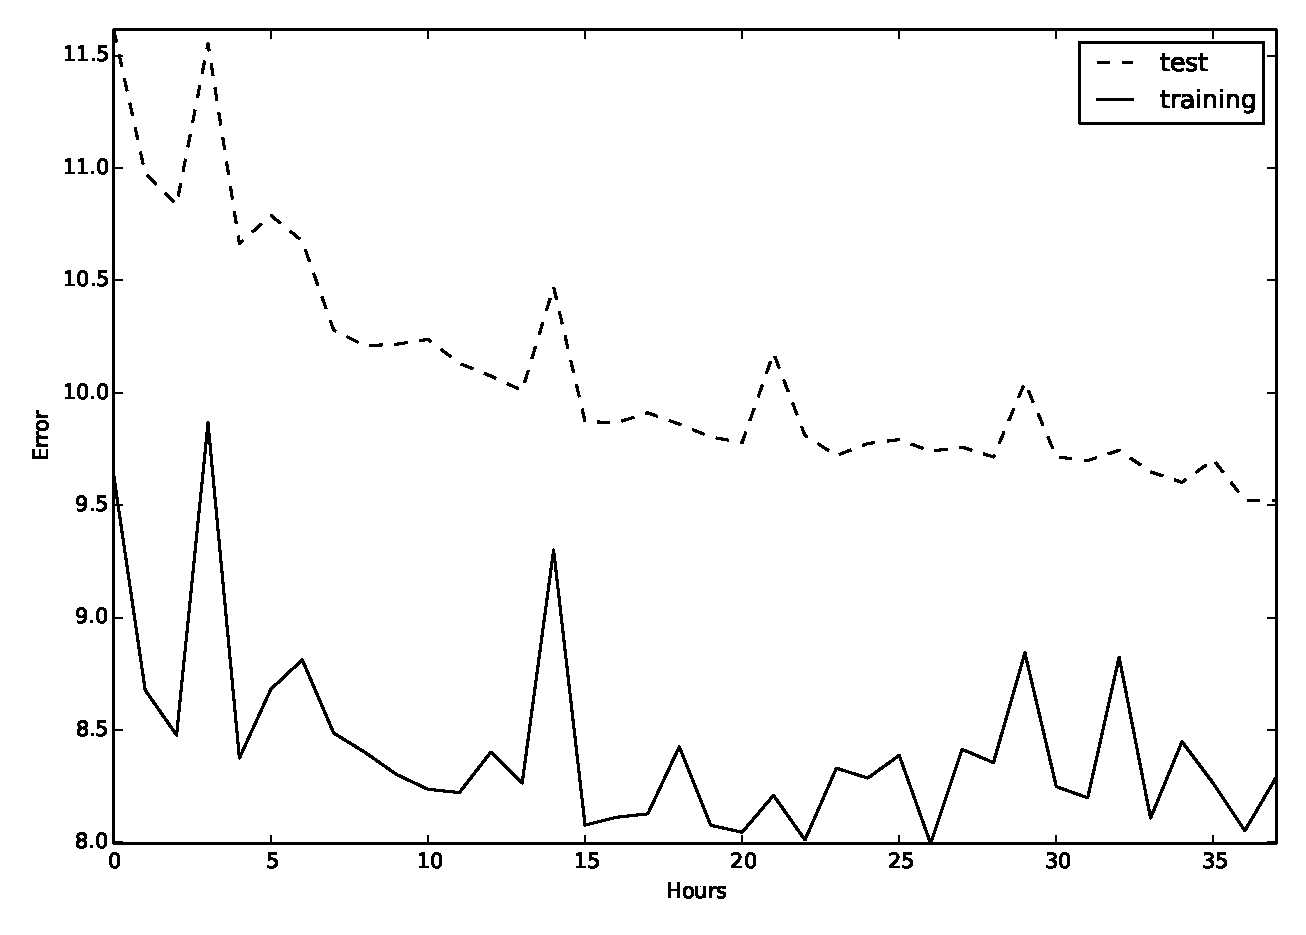
\epsfig{file=images/trainingCurve.eps, width=\columnwidth}
\caption{Training curve of the hybrid model with 80 hidden neurons}
\end{figure}
This project used Python and Pybrain \cite{schaul2010} to construct the planned ANN and the R forecast package of Rob J. Hyndman \cite{hyndman2007automatic}. 

\subsection{Outlier detection}

According to Chebschev's theorem \cite{amidan2005data}, almost all the observations in a data set of system states falls into the interval $[\mu - 3\sigma, \mu+3\sigma]$, where $\mu$ and $\sigma$ are respectively the mean and standard deviation of the data set, and the data points outside this interval are declared outliers. In this paper the ANN is used to predict the gas consumption, for this reason a point will be considered outlier if it will fall outside the $95\%$ confidence interval\footnote{For the following description user \textit{fabee} of CrossValidated.com needs to be cited \url{https://stats.stackexchange.com/questions/78079/confidence-interval-of-rmse}} expressed for the RMSE. If it is assumed that the difference between the actual values $x_i$ and the predicted value $\hat{x_i}$ have:
\begin{equation}
\hat{x}_{i}-x_{i}	\sim	\mathcal{N}\left(0,\sigma^{2}\right)
\end{equation}
\begin{itemize}
\itemsep0em
  \item mean zero.
  \item follow a Normal distribution (it is assumed that it holds for the large amount of data utilized).
  \item and all have the same standard deviation $\sigma$.
\end{itemize}
\begin{equation}
\label{equation:preRMSE}
\hat{x}_{i}-x_{i}	\sim	\mathcal{N}\left(0,\sigma^{2}\right)
\end{equation}
it is possible to say that \cref{equation:preRMSE} follows a $\chi_{n}^{2}$ distribution with $n$ degrees of freedom. Which means:
\begin{align}
P\left(\chi_{\frac{\alpha}{2},n}^{2}\le\frac{n\mbox{RMSE}^{2}}{\sigma^{2}}\le\chi_{1-\frac{\alpha}{2},n}^{2}\right)	=	1-\alpha\\
\Leftrightarrow P\left(\frac{n\mbox{RMSE}^{2}}{\chi_{1-\frac{\alpha}{2},n}^{2}}\le\sigma^{2}\le\frac{n\mbox{RMSE}^{2}}{\chi_{\frac{\alpha}{2},n}^{2}}\right)	=	1-\alpha\\
\Leftrightarrow P\left(\sqrt{\frac{n}{\chi_{1-\frac{\alpha}{2},n}^{2}}}\mbox{RMSE}\le\sigma\le\sqrt{\frac{n}{\chi_{\frac{\alpha}{2},n}^{2}}}\mbox{RMSE}\right)	=	1-\alpha.
\end{align}
Therefore
\begin{equation}
\left[\sqrt{\frac{n}{\chi_{1-\frac{\alpha}{2},n}^{2}}}\mbox{RMSE},\sqrt{\frac{n}{\chi_{\frac{\alpha}{2},n}^{2}}}\mbox{RMSE}\right]
\end{equation}

\section{Experimental Evaluation}
The ANN has been trained with early stopping, with a fixed number of training epochs (phases) or stopping the training when the validation error rate was increasing. All the results showed are obtained from a k-fold cross-validation techniques, where the network was trained $k$ times, each time leaving out a subset of data from training in order to test the ANN. The results of the $k$ tests, were divided by $k$.

%methods, mape etc

Although most the Mean Absolute Percentage Error (MAPE) is considered a standard for examining the quality of the models prediction of energy load, it is an adequate error measure only if the loss function were linear and recent studies demonstrated it is not \cite{kalogirou2006artificial}\cite{kajl2000evaluation}. Moreover the percentage error is infinite if there are zero values on the series, frequent in intermittent data and in consumption data, and it puts a heavier penalty on positive errors than on negative errors \cite{hyndman2006another}. Because of these disadvantages, this paper will only consider the minimization of the Root Mean Square Error (RMSE), which penalize large errors, as suggested in \cite{yao2005method}. As suggested in \cite{hippert2001neural}, for every experiment also the Mean Absolute Error (MAE) will be calculated. 

\begin{equation}\operatorname{MAPE}\footnote{MAPE errors will be calculated only on the non-zero values, to avoid the problems described before.}=\frac{1}{n}\sum_{i=1}^{n} \frac{|Y_{i} - \hat{Y_i}|}{Y_{i}} \times 100 \end{equation}

\begin{equation}\operatorname{RMSE}=\sqrt{\frac{1}{n}\sum_{i=1}^n(\hat{Y_i} - Y_i)^2}\end{equation}

\begin{equation}\operatorname{MAE}=\frac{1}{n}\sum_{i=1}^n \left| \hat{Y_i}-Y_i\right|\end{equation}

\noindent where $\hat{Y}$ is the vector of the $n$ predictions and $Y$ is the vector of the true values.


\subsection{Synthetic experiments}
The method is tested with synthetic generated data. Two days outliers were generated by different algorithms. In the first one the real consumption was modified by a random value, simulating the system measurement/control malfunction which makes the consumption bouncing up and down (see \cref{equation:synt1}). The second synthetically created day was created adding $50 m^3$ of gas consumption to the real one, creating a pattern which simulates a strange behaviour and/or a malfunction of the heating system (see \cref{equation:synt2}).

\begin{equation}G(t)= G(t)+v*30\label{equation:synt1} \end{equation}
where 
\begin{align*}v \sim \mathcal{N} (0,\sigma^2) \end{align*}

\begin{equation}G'(t)= G'(t)+50\label{equation:synt2} \end{equation}

\begin{figure*}
\centering
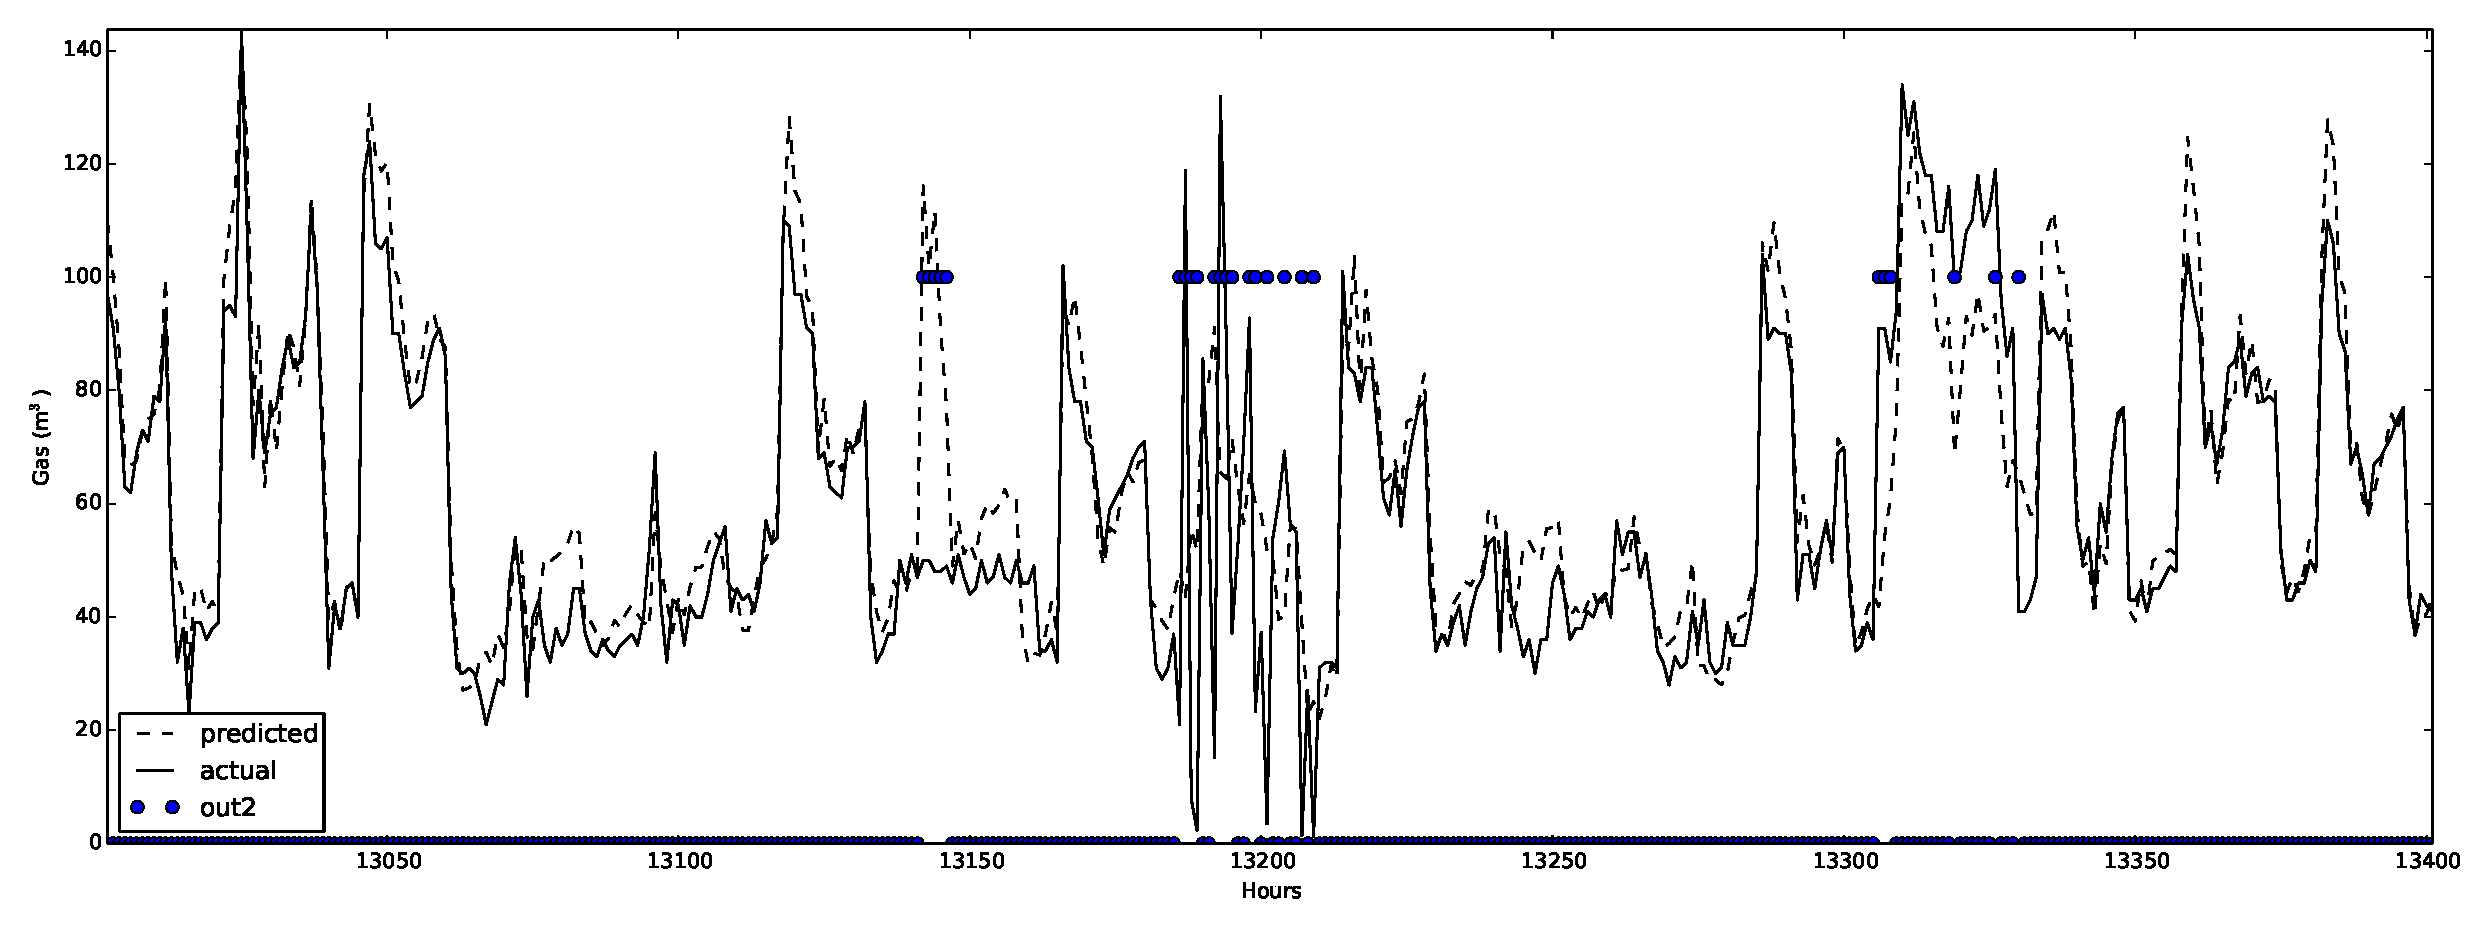
\includegraphics[width=\textwidth]{images/outliersSynt.eps}
\caption{Outlier detection with synthetic generated data. The circle represents the hours where an outlier is detected.}
\label{fig:outlierSynt}
\end{figure*}

The two outliers were correctly detected, as it can be seen in \cref{fig:outlierSynt}.

\subsection{Measured data experiments}
The method is also tested with measured data, coming from a different type of the day. For example the gas consumption of a week-end was placed in a week-day, simulating a holiday. The purpose of this test was to show that the unusual pattern was detected. In \cref{fig:outlierReal} it can be seen that the outlier mechanism works perfectly when the Sunday gas consumption is placed in a weekday. 

\begin{figure*}
\centering
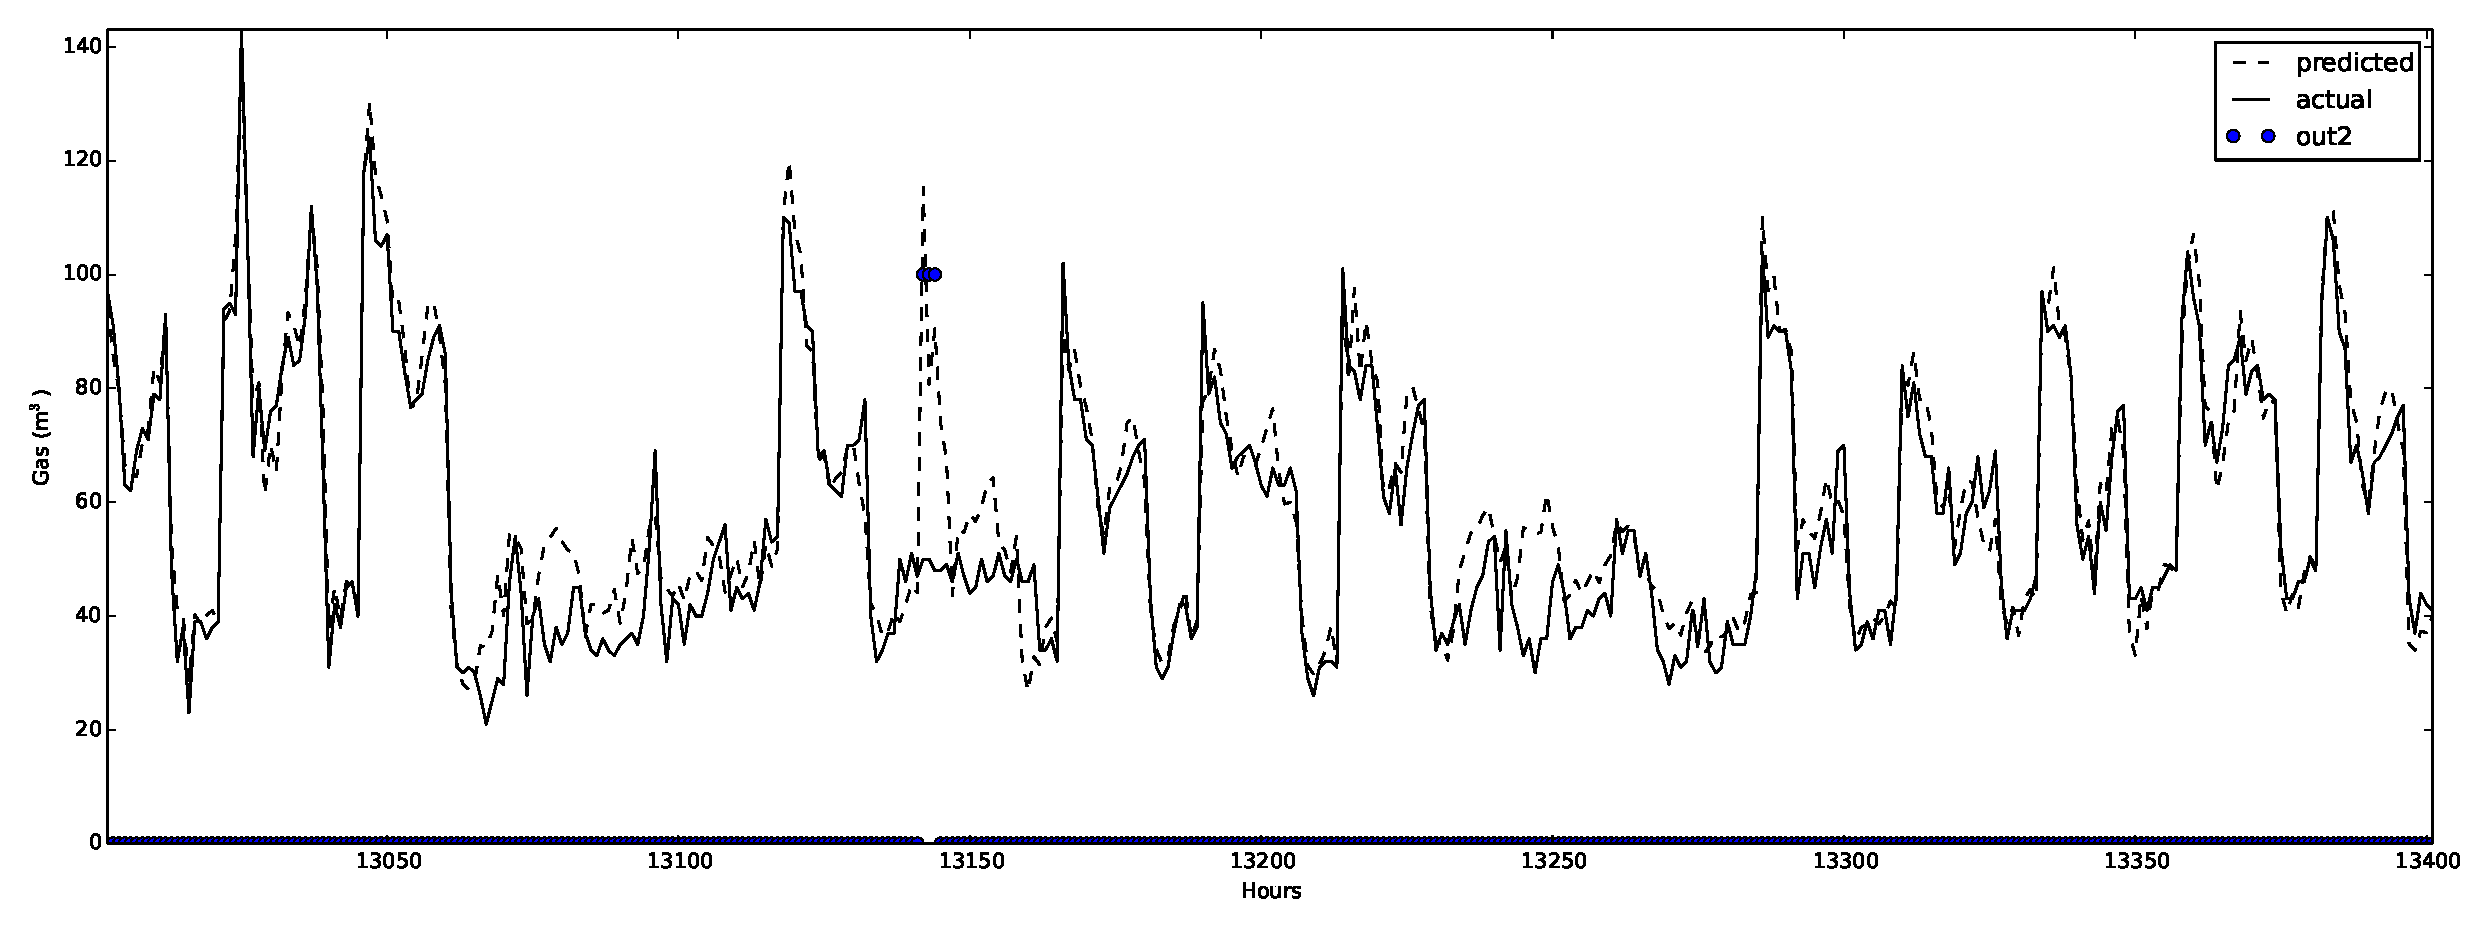
\includegraphics[width=\textwidth]{images/outliersReal.eps}
\caption{Outlier detection where the gas consumption of a weekday was replaced by a Sunday one. The (three) circles represent the outliers detected by the system.}
\label{fig:outlierReal}
\end{figure*}

The outlier was correctly detected, as it can be seen in \cref{fig:outlierReal}. The robustness of the design was proved with different building, listed in \cref{tab:dataset}.

\section{Conclusion}

Any model can't be treating accurately all the situations for a large amount of historical load data. The irregular fluctuation of the gas consumption was hardly predictable, for this reason the ANN model needed help from a classic linear model like ARIMA. Although other papers presented similar models to forecast electric consumption, the hybrid model presented here, is almost unique because it focuses to forecast short-term gas consumption, which are very irregular and not easily predictable with classic methods. Since the predictor is very accurate (with RMSE of $7.995$), the outlier mechanism is able to easily detect strange behaviours defining a threshold value in the confidence interval without the need to possess previous example of outliers.



%Errori nelle domeniche alti

% future works

%\end{document}  % This is where a 'short' article might terminate

%ACKNOWLEDGMENTS are optional
\section{Acknowledgments}
This work and internship was economically supported by Universita' degli studi di Trento.

%
% The following two commands are all you need in the
% initial runs of your .tex file to
% produce the bibliography for the citations in your paper.
\bibliographystyle{abbrv}
\bibliography{sigproc}  % sigproc.bib is the name of the Bibliography in this case
% You must have a proper ".bib" file
%  and remember to run:
% latex bibtex latex latex
% to resolve all references
%
% ACM needs 'a single self-contained file'!
%
%APPENDICES are optional
\appendix
%Appendix A
\section{Sources}
``Very often scientific studies rely on complex textual explanations of what has been done to analyse the data that can overwhelm the reader that has to accept them as an act of faith", as stated in \cite{reproducibility}. To avoid this, the author provides all the sources through this website: \url{https://github.com/denadai2/energyUva}. The raw data are protected by privacy of the Hogeschool van Amsterdam. The Universiteit van Amsterdam is working to make them available to achieve total reproducibility.

%\balancecolumns

\balancecolumns % GM July 2000
% That's all folks!
\end{document}
